%%%%%%%%%%%%%%%%%%%%%%%%%%%%%%%%%%%%%%%%%
% MODELE DE MANUSCRIT DE THESE 
% DE L'UNIVERSITE PARIS CITE
% OFFICIEL

% LaTeX Template
% Version overleaf (14/10/2023) 
% Format BOOK
% Par Aleksandra SAVINA, PhD
%%%%%%%%%%%%%%%%%%%%%%%%%%%%%%%%%%%%%%%%%


%----------------------------------------------------------------------------------------
%	PREAMBULE // PACKAGES AND OTHER DOCUMENT CONFIGURATIONS
%----------------------------------------------------------------------------------------
\documentclass[a4paper,12pt,twoside,french]{book}
[a4paper,12pt,twoside]
\usepackage[utf8]{inputenc}
\usepackage[T1]{fontenc}
\usepackage{babel}
%	MARGIN SETTINGS
\usepackage[a4paper,left=3cm,right=2.5cm,top=3cm,bottom=3cm, twoside]{geometry}

\usepackage{xcolor}
\usepackage{stmaryrd}
\usepackage{amssymb}
\usepackage{amsmath}
\usepackage{libertine}

%\usepackage{cite}
\usepackage{hyperref} % for references (\ref, \label), url
\hypersetup{
    colorlinks=true,
    linkcolor=black,
    filecolor=black,      
    urlcolor=black,
    citecolor=black,
    pdfpagemode=FullScreen,
    }
\usepackage[
    %backend=biber, 
    natbib=true,
    style=numeric,
    sorting=none
]{biblatex} %Imports biblatex package

\addbibresource{biblio.bib} %Import the bibliography file

\usepackage{graphicx} % to include images
%\usepackage[pdftex]{graphicx}
\graphicspath{ {figures/} }
\usepackage{caption}
\usepackage{subcaption}
\usepackage{float}
\usepackage{multirow}
\usepackage{array, multirow, tabularx}
\usepackage{booktabs}
\usepackage{longtable}
\usepackage{apalike}
\usepackage{minitoc}
\usepackage{tikz}
\usepackage{fancyhdr}
\pagestyle{fancy}
\usepackage[strict]{changepage}
\usepackage{siunitx}
\selectlanguage{french}%

\usepackage{enumitem}
\usepackage{epigraph}
%\usetikzlibrary{shadows.blur}
\usepackage{lscape}
\usepackage{titletoc}
\usepackage{mdframed}

\usepackage{tabu}
\usepackage{pdfpages}

\usepackage{arydshln}
%\usepackage[nonumberlist]{glossaries}
\usepackage{calc}
\usepackage[]{titlesec} 
\definecolor{linkColor}{HTML}{32a852}
%\usepackage[colorlinks=true,citecolor=linkColor,linkcolor=black]{hyperref}

\addto\captionsfrench{%
  \renewcommand{\listfigurename}{Liste des figures}%
}


%%%%%%%%%%%%%%%%%%%%%%%%%%%%%%%%%%%%%%%%%%%%%%%%%%%%%%%%%%%%%%%%%%%%%%%%%%
%%%%%%%%%%%%%%%%%%%%%%%%%%%%%%%%%%%%%%%%%%%%%%%%%%%%%%%%%%%%%%%%%%%%%%%%%%

\usepackage{sectsty}
%\sectionfont{\color{CentraleRed}}  % sets colour of sections
%\subsectionfont{\color{uclablue}}  % sets colour of subsections, ou gray, teal 
\definecolor{darkseagreen}{rgb}{0.56, 0.74, 0.56}
\usepackage{lipsum}

\title{NMR global data Version2}
\author{Aleksandra Savina}
\date{October 2022}


%----------------------------------------------------------------------------------------
%	HEADERS AND FOOTERS
%----------------------------------------------------------------------------------------

%\fancyhead[RO]{\scshape \leftmark}
%\fancyhead[L]{\scshape \righttmark}
\fancyhead{} % clear all header fields
\fancyfoot{} % clear all footer fields
%\fancyhead[LE,RO]{\slshape \rightmark}
\fancyfoot[C]{--~\thepage~--}

\usepackage{emptypage}

%\leftmark : adds name and number of the current top-level structure (for example, Chapter for reports and books classes; Section for articles ) in uppercase letters.
% \rightmark : adds name and number of the current next to top-level structure (Section for reports and books; Subsection for articles) in uppercase letters.

%%%%%%Glossaire
%\usepackage{glossaries}
\usepackage[acronym,xindy,toc]{glossaries} % nomain, if you define glossaries in a file, and you use \include{INP-00-glossary}
%[nomain,acronym,xindy,toc]
\makeglossaries

\usepackage[xindy]{imakeidx}
\makeindex
%\input{auxilliaires/glossaire}
%%%%%%%%%%%%%%%%%%%%%%%%%%%%%%%%%%%%%%%%%%%%%%%%%%%%%%%%%%%%%%%%%%%%%%%%%%
%%%%%%%%%%%%%%%%%%%%%%%%%%%%%%%%%%%%%%%%%%%%%%%%%%%%%%%%%%%%%%%%%%%%%%%%%%
%----------------------------------------------------------------------------------------
%	DOCUMENT
%----------------------------------------------------------------------------------------
\begin{document}

%\maketitle
%----------------------------------------------------------------------------------------
%	TITLE PAGE
%----------------------------------------------------------------------------------------
	\begin{titlepage}
		\begin{center}
			\begin{tabular}{c@{\hskip 7cm}c@{\hskip 1cm}}
				
\includegraphics[height=2.5cm]{figures/PageTitre/UParisCitelogo.jpg} &
				%si autre logo : 
\includegraphics[height=2.3cm]{figures/PageTitre/logo_ic_2021.jpg}
			\end{tabular}
		\end{center}
	
		\begin{center}
		
\vspace*{.03\textheight}
\textsc{\LARGE Université Paris Cité}\\[0.2cm] % Univ name
		\large École doctorale [Nom et numéro identifiant]\\
		  Laboratoire \\ 
        %Équipe de recherche\\
  
  			\vfill
 
	 		\rule{\textwidth}{0.8pt} \\ % Horizontal line
	 		\vspace{10pt}
	 		 { \LARGE \bfseries Insérer le titre de la thèse ici \textit{(dans la langue de rédaction)}} % Thesis title
	 		 \vspace{10pt}
	 		 \rule{\textwidth}{0.8pt} \\ % Horizontal line
		\end{center}
		
		\vfill
		% Author and supervisor	
		\begin{center}
			Par \textsc{\Large Prénom NOM}\\[1cm] 
			Thèse de doctorat de \textsc{\large spécialité}\\[1.2cm]
			Dirigée par \textsc{\large Prénom NOM}\\[0.2cm]
            Et par \textsc{\large Prénom NOM} (en cas de co-direction et non de co-encadrement) \\[0.2cm] 
			Présentée et soutenue publiquement/à huis clos le JJ/MM/AAAA %renseigner la date et choisir le type de soutenance
		\end{center}
		
		\vspace{1cm}
Devant un jury composé de : %(indiquer le jury complet) 		
		\begin{center}
			\begin{tabular}{l@{\hskip 1cm}l@{\hskip 1cm}l}
				\textsc{Prénom NOM, Prof. HDR} & Université de Namur, Belgique  & Rapporteur \\
				\textsc{Prénom NOM, DR}  & Université de Ville &Rapportrice \\
				\textsc{Prénom NOM, CR-HDR}  & Université Paris Cité &Examinatrice\\
                \textsc{Prénom NOM, DR}  & Université de Y &Examinateur\\
				\textsc{Prénom NOM, MCF}  &Université Paris Cité  &Examinatrice \\
				\textsc{Prénom NOM, PU-PH}  &Université Paris Cité &Membre invité \\
				\textsc{Prénom NOM, PhD}  &Entreprise X &Membre invité \\
				\textsc{Prénom NOM, MCF-HDR}  &Université Paris Cité &Directeur de thèse \\
			\end{tabular}\\[1cm]
		\end{center}

	\newpage %page de garde vide
	\thispagestyle{empty} %page de garde vide
	\end{titlepage}

%\renewcommand{\chaptermark}[1]{\markboth{\textsc{#1}}{}}
\renewcommand{\chaptermark}[1]{\markboth{#1}{}}


\frontmatter % numérote les pages en chiffres romains jusqu'a la commande mainmatter

%----------------------------------------------------------------------------------------
%	RESUME ET ABSTRACT PAGE
%----------------------------------------------------------------------------------------
\chapter*{Résumé}
\addcontentsline{toc}{chapter}{Résumé} 

\begin{mdframed}
\vspace{-.25cm}
\paragraph*{Titre:} Insérer le titre de la thèse ici \textit{(en français)}.

\begin{small}
\vspace{-.25cm}
\paragraph*{Mots clefs:} Mot clef ; Mot clef ; Mot clef; Mot clef ;  Mot clef ; Mot clef

\vspace{-.5cm}
\setlength{\columnsep}{12pt} % I want the columnsep to be wider only on this page.
\begin{multicols}{2}
\paragraph*{Résumé:} 
Utilisation d'une abréviation de cette manière lorsque le mot apparaît pour la première fois dans le document : "le rat-taupe nu (\acrshort{RTN}) constitue un modèle mammifère présentant peu de signes liés à l’âge." 
Par la suite, le mot est utilisé par sa seule abréviation : " L'objectif de cette thèse est donc d'explorer les caractéristiques et les mécanismes sous-tendant la possible résistance cutanée du \acrshort{RTN} au vieillissement."

\lipsum[1-4]


\end{multicols}
\end{small}
\end{mdframed}

\clearpage 

\begin{mdframed}
\vspace{-.25cm}
\paragraph*{Title:} Insert thesis title here (in English).

\begin{small}
\vspace{-.25cm}
\paragraph*{Keywords:}  Keyword ; Keyword ; Keyword ; Keyword ;  Keyword ; Keyword ; Keyword 

\vspace{-.5cm}
\setlength{\columnsep}{12pt} % I want the columnsep to be wider only on this page.
\begin{multicols}{2}
\paragraph*{Abstract:}
\lipsum[1-5]


\end{multicols}
\end{small}
\end{mdframed}
	
\newpage
\thispagestyle{empty}
\mbox{}
\newpage %résumé en francais
%\chapter*{Abstract}
\addcontentsline{toc}{chapter}{Abstract} 

%\thispagestyle{plain}
Résumé, mots-clés et titre en anglais
Obligatoire
\begin{itemize}
    \item Résumé : entre 1700 et 4000 caractères (espaces compris). Éviter d’inclure des formules dans le résumé.
    \item Mots-clés : pas plus d'une dizaine. Veiller à être précis.
    \item es éléments sont utilisés pour le signalement des thèses dans les catalogues et sur des portails locaux, nationaux ou internationaux.
    \item ajouter les logos ?
\end{itemize} ...

    

 %résumé en anglais

%----------------------------------------------------------------------------------------
%	QUOTATION PAGE ou DEDICACE
%----------------------------------------------------------------------------------------
\clearpage
\vspace*{0.2\textheight}

\begin{quote}
\textbf{Exemple de citation :} \\
Comme lorsque la brume se dissipe, \\ le regard peu à peu trouve une figure\\ dans la vapeur dont les airs sont épaissis, \\ ainsi, perçant l'élément lourd et obscur\\ à mesure que nous approchions du bord, \\l'erreur me quittait ...
\end{quote} \bigbreak

\hfill 
L’Enfer – Chant XXXI, La Divine Comédie, Dante Alighieri

%----------------------------------------------------------------------------------------


%----------------------------------------------------------------------------------------
%	ACKNOWLEDGEMENTS
%----------------------------------------------------------------------------------------
\chapter*{Remerciements}
\addcontentsline{toc}{chapter}{Remerciements} 

Je remercie xxx \lipsum[66]

\bigskip

Je remercie xxx \lipsum[66]

\bigskip

Je remercie également \lipsum[66]

\bigskip

Je remercie xxx \lipsum[66]

\bigskip

Je remercie xxx \lipsum[66]

\bigskip

Je remercie xxx \lipsum[66]

\bigskip

Je remercie xxx \lipsum[66]


\newpage
\thispagestyle{empty}
\mbox{}
\newpage


%----------------------------------------------------------------------------------------
%	LIST OF CONTENTS/FIGURES/TABLES PAGES
%----------------------------------------------------------------------------------------
%\setcounter{secnumdepth}{3} % organisational level that receives a numbers
%\setcounter{tocdepth}{3}
\tableofcontents % Prints the main table of contents
\listoffigures % Prints the list of figures
\addcontentsline{toc}{chapter}{Liste des figures}
\listoftables % Prints the list of tables
\addcontentsline{toc}{chapter}{Liste des tableaux}
\newpage


%----------------------------------------------------------------------------------------
%	Liste des abréviations-
%----------------------------------------------------------------------------------------
%\chapter*{Liste des abréviations}
%\addcontentsline{toc}{chapter}{Liste des abréviations} 

\printglossary[type=\acronymtype, title=Acronyms,toctitle=Acronyms]

\newacronym{CFD}{CFD}{Computational Fluid Dynamics}
\newacronym{CNN}{CNN}{Convolutional Neural Networks}
\newacronym{DL}{DL}{Deep Learning}
\newacronym{GDL}{GDL}{Geometric Deep Learning}
\newacronym{GNN}{GNN}{Graph Neural Networks}
\newacronym{ML}{ML}{Machine Learning}
\newacronym{MLP}{MLP}{Multi-Layer Perceptron}
\newacronym{MSE}{MSE}{Mean Squared Error}
\newacronym{NACA}{NACA}{National Committee for Aeronautics}
\newacronym{NASA}{NASA}{National Aeronautics and Space Administration}
\newacronym{PDE}{PDE}{Partial Differential Equations}
\newacronym{PINN}{PINN}{Physics-Informed Neural Networks}
\newacronym{RANS}{RANS}{Reynolds-Averaged Navier–Stokes}
\newacronym{RAS}{RAS}{Reynolds-Averaged Simulation}
\newacronym{TMR}{TMR}{Turbulence Modeling Resource}


% --------------------------------------------------------------
%                         Début du corps
% --------------------------------------------------------------

\mainmatter
\setlength{\parskip}{.7em}

%\titlespacing*{\section}{0pt}{.9em}{.8em}
\renewcommand{\baselinestretch}{1.1}

\fancyhead[RO]{\leftmark}
\fancyhead[LE]{\textsc{\chaptername~\thechapter}}

%\chapter*{Introduction}
\fancyhead{} % clear all header fields
\fancyhead[OL]{\textsc{Avant-propos}}
\chapter*{Avant-propos} % Main chapter title
\addcontentsline{toc}{chapter}{Avant-propos}  

%Le but de l'avant-propos est d'améliorer les conditions dans lesquelles les membres d’un jury, vont pouvoir l’apprécier.
%\textbf{C’est une partie facultative du travail de recherche dans laquelle l’auteur peut expliquer les raisons qui l’ont incité à étudier le sujet en question, tout en exposant le but poursuivi et les difficultés rencontrées en cours de recherche.}

\lipsum[66]


\subsubsection*{Titre de la sous-section}

\lipsum[66]

\lipsum[70]


\subsubsection*{Titre de la sous-section}

\lipsum[70]


\subsubsection*{Titre de la sous-section}

\lipsum[66]

\begin{itemize}
    \item Lorem ipsum dolor sit amet, consectetur adipiscing elit ?
    \item Lorem ipsum dolor sit amet, consectetur adipiscing elit ? 
    \item Lorem ipsum dolor sit amet, consectetur adipiscing elit ?
\end{itemize}

\lipsum[70]
 %partie introduction ou avant-propos

\fancyhead{} % clear all header fields

\fancyhead[RO]{\leftmark}
\fancyhead[LE]{\textsc{\chaptername~\thechapter}}

\chapter{Titre du chapitre} % Main chapter title

%----------------------------------------------------------------------------------------
%	SECTION 
%----------------------------------------------------------------------------------------
\section{Titre de la section}


\subsection{Titre de la sous-section : abréviations, paragraphes, citations, figures et tableaux}
\subsubsection{Titre de la sous-sous-section : utilisation des citations et abréviations}

La première \textbf{citation} : \cite{Ruppell1842}. %(\acrshort{rtn})
La deuxième et troisième citations : \cite{Faulkes2013,Faulkes2021}.

\textbf{Voici l'exemple pour une abréviation.}
Union Internationale pour la Conservation de la Nature apparaît pour la première fois dans le texte sous sa forme complète puis l'abréviation sera utilisée : l’\acrshort{IUCN}. La forme longue de cette abréviation doit être précisée dans la partie "abréviations" dans "auxilliaires". Ainsi, lorsque la forme courte apparaîtra, les pages seront référencées.
\textbf{Autre exemple }: La jonction dermo-épidermique (\acrshort{JDE}) est une membrane basale (\acrshort{MB}) spécifique.


\subsubsection{Titre de la sous-sous-section : rédiger avec des paragraphes}

\paragraph{Titre du paragraphe.} 

\lipsum[60]

\begin{figure}[h]
\centering

\includegraphics[scale=0.2]{figures/chap1/SiegeUP_1920-1.jpg} %pour fixer l'échelle.
\caption[Titre de la figure qui va apparaître dans la table]{Titre de la figure qui va apparaître sous la figure dans le document. Extrait de \cite{Smith2021-wv}.}
\label{fig:siegeUP}
\end{figure}



\subsubsection{Titre de la sous-sous-section : faire référence à une figure et lettres grecques}

\textbf{Référence à une figure} dans le texte : (figure \ref{fig:siegeUP}). 
Exemples des \textbf{lettres grecques} : $\alpha$, $\beta$, $\gamma$, $\delta$


%figure dans le document
\begin{figure}[ht]
\centering

\includegraphics[scale=0.35]{figures/chap1/faculte-upc.png} %pour fixer l'échelle.
\caption[Titre de la figure qui va apparaître dans la table]{Titre de la figure qui va apparaître sous la figure (extrait ou adapté de \cite{Faulkes2021}).}
\label{fig:faculteUPC}
\end{figure}


\subsection{Titre de la sous-section}
\label{ajout-du-label-pour-faire-reference-a-la-sous-section}
 


\begin{table}[tb]%[!ht]
    \raggedleft
    \caption{Liste des 5 génomes officiels d'\textit{Heterocephalus glaber} selon le NCBI.}
    \begin{tabular}{llllp{4cm}}
    \hline \hline
        \textbf{Assembly Name} & \textbf{Size (Mb)} & \textbf{Level} & \textbf{Date} & \textbf{Annotation Name} \\ \hline
        HetGla\_female\_1.0 & 2,618 & Scaffold & Mar, 2012 & NCBI RefSeq \\ \hline
       HetGla\_1.0 & 2,644 & Scaffold & Nov, 2011 & Annotation submitted by Beijing Genomics Institute \\ \hline
      Heter\_glaber.v1.7\_hic\_pac & 3,042 & Scaffold & Sep, 2020 & ~ \\ \hline
        Naked mole-rat maternal & 2,500 & Chromosome & Aug, 2022 & ~ \\ \hline
       Naked mole-rat paternal & 2,499 & Chromosome & Aug, 2022 & ~ \\ \hline \hline
    \end{tabular}
\end{table}


\subsubsection{Titre de la sous-sous-section : tables, tableaux et tableaux sur 2 pages}
Le tableau \ref{tab-dom-et} présente xxx.

\lipsum[60]

%\small
\begin{center}
\footnotesize
\begin{longtable}{p{3cm}p{10.5cm}}
\caption{Titre de la table longue (sur 2 pages).} \label{tab-dom-et} \\
\hline \hline \multicolumn{1}{l}{\textbf{Domaine d’étude}} & \multicolumn{1}{p{10cm}}{\textbf{Principales caractéristiques d’intérêt pour ces domaines d’études}} \\ \hline 
\endfirsthead

\multicolumn{2}{l}%
{{\bfseries \tablename\ \thetable{} -- suite de la page précédente}} \\
\hline \multicolumn{1}{l}{\textbf{Domaine d’étude}} & \multicolumn{1}{p{10cm}}{\textbf{Principales caractéristiques d’intérêt pour ces domaines d’études}} \\ \hline 
\endhead

\hline \multicolumn{1}{c}{{Suite à la page suivante}} \\ \hline
\endfoot

\hline \hline
\endlastfoot

Coopération sociale             &   Eusocialité \cite{Ruppell1842, Faulkes2013}, rôle insaisissable de la prolactine \cite{Faulkes2013}. \\
Endocrinologie et \newline Reproduction   &   Régulation phosphocalcique et de la glycémie singulière, utilisation privilégiée du cortisol, inhibition de l’axe gonadotrope, report de la puberté, pas de ménopause \cite{Faulkes2013}.   \\
Oncologie                       & Résistance aux cancers : plusieurs formes de cancers spontanés ou expérimentalement induits, caractéristiques génomiques uniques et des adaptations moléculaires compatibles avec la résistance au cancer \cite{Faulkes2013}.      \\
Hypoxie et \newline hypercapnie          &   Tolérance accrue à l'hypoxie, survie pendant des heures à 3\% d'O2 \cite{Faulkes2013}, survie de 18 minutes en anoxie \cite{Faulkes2013}, évolution dans un environnement confiné avec une forte densité animale \cite{Faulkes2013}. Réorganisation du métabolisme pour tolérer un environnement faible en oxygène \cite{Faulkes2013}. Niveau élevé d'activation du facteur 1$\alpha$ inductible de l'hypoxie (HIF-1$\alpha$), d'expression du facteur A de croissance endothéliale vasculaire (VEGFA), du NF$\kappa$B et de plusieurs protéines impliquées dans les fonctions neuroprotectrices pendant les conditions hypoxiques \cite{Faulkes2013}. Réponses ventilatoires hypoxiques et hypercapniques diminuées, pas d'oedème pulmonaire \cite{Faulkes2013}. \\
Somatosensoriel                 & Organe voméro-nasal peu développé, vision rudimentaire, rôle des vibrisses et poils sensoriels dans son orientation spatiale, organisation corticale somatosensorielle, sensibilité auditive originale \cite{Faulkes2013}.     \\ 
Somatosensoriel                 & Organe voméro-nasal peu développé, vision rudimentaire, rôle des vibrisses et poils sensoriels dans son orientation spatiale, organisation corticale somatosensorielle, sensibilité auditive originale \cite{Faulkes2013}.     \\ 
Somatosensoriel                 & Organe voméro-nasal peu développé, vision rudimentaire, rôle des vibrisses et poils sensoriels dans son orientation spatiale, organisation corticale somatosensorielle, sensibilité auditive originale \cite{Faulkes2013}.     \\ 
Somatosensoriel                 & Organe voméro-nasal peu développé, vision rudimentaire, rôle des vibrisses et poils sensoriels dans son orientation spatiale, organisation corticale somatosensorielle, sensibilité auditive originale \cite{Faulkes2013}.     \\ 
Système X & Système et détails \cite{Faulkes2013}.   \\
\end{longtable}
\end{center}





%----------------------------------------------------------------------------------------
%	SECTION 
%----------------------------------------------------------------------------------------
\clearpage 



\section{Titre de la section}

\subsection{Titre de la sous-section}

\subsection{Titre de la sous-section}


%----------------------------------------------------------------------------------------
%	SECTION 
%----------------------------------------------------------------------------------------
\chapter{Titre du chapitre} % Main chapter title


%----------------------------------------------------------------------------------------
%	SECTION 
%----------------------------------------------------------------------------------------
\section{Titre de la section}
%-----------%-----------
%	SOUS-SECTION 
%-----------%-----------
\subsection{Titre de la sous-section}

%-----------
%	SOUS-SOUS-SECTION 
%------------
\subsubsection{Titre de la sous-sous-section}
%-----------
%	SOUS-SOUS-SECTION 
%------------
\subsubsection{Titre de la sous-sous-section}


%-----------%-----------
%	SOUS-SECTION 
%-----------%-----------
\subsection{Titre de la sous-section}

%-----------
%	SOUS-SOUS-SECTION 
%------------
\subsubsection{Titre de la sous-sous-section}

%-----------
%	SOUS-SOUS-SECTION 
%------------
\subsubsection{Titre de la sous-sous-section}

%-----------%-----------
%	SOUS-SECTION 
%-----------%-----------
\subsection{Titre de la sous-section}


%----------------------------------------------------------------------------------------
%	SECTION 
%----------------------------------------------------------------------------------------


%-----------------------------------
%	SECTION 
%-----------------------------------
\section{Titre de la section}




%-----------------------------------
%	SECTION 
%-----------------------------------

\section{Titre de la section}

\begin{table}[h]%[!ht]%[tb]
\footnotesize
    \caption{Titre de la table.}
    \begin{tabularx}{1\textwidth}{
     >{\raggedright\arraybackslash}X 
     >{\raggedright\arraybackslash}X 
     >{\raggedright\arraybackslash}X  }  \hline \hline
        \textbf{ }                      & \textbf{Souris}                       & \textbf{Humain} \\ \hline
        \textbf{Cycle pilaire}          & $\approx$ \num{3} semaines            & Variable: région-dépendant \\ 
        \textbf{Pilosité et densité}   & Élevées : \num{1000}/\unit{\square\milli\metre}                  & Faibles : \num{25}/\unit{\square\milli\metre} \\ 
        \textbf{Épaisseur épidermique}  & Fine, \num{2}-\num{5} couches, \SI{10}{\micro\metre}           & Épaisse, $>$\num{10} couches, \num{60}-\SI{90}{\micro\metre}  \\ 
        \textbf{Papilles dermiques}     & Absence                               & Présence \\ 
        \textbf{Pigmentation}           & Follicule pilleux                     & Épiderme interfolliculaire \\ 
        \textbf{Renouvellement EIF} & \num{8}-\num{10} jours                         & \num{28}-\num{39} jours \\ 
        \textbf{Épaisseur dermique}     & Plus fine                              & Plus épaisse \\ 
        \textbf{Glandes sudorales apocrines} & Absence dans la peau             & Présence dans les régions cutanées axillaires, inguinales et périanales \\ 
        \textbf{Propriétés biomécaniques } & Mince, souple, lâche               & Épaisse, relativement rigide, adhérante aux tissus sous-jacents. \\ 
        \textbf{Épaisseur de l'hypoderme} & Dépendante du cycle pillaire         & Peu variable  \\ 
        \textbf{Couche musculaire sous-cutanée} & présence du \textit{panniculus carnosus}  & Présence uniquement dans la région du cou (platysma) \\
        \textbf{Principale méthode de cicatrisation} & Contraction              & Formation de tissu de granulation et réépithélialisation \\ 
        \textbf{Nombre de couches}      & \num{3}                                     & \num{3} \\ 
        \textbf{Lymphocytes T (EIF)}          & DETC                  & a/b T cells \\ \hline \hline
    \end{tabularx}
    \label{table:diff-souris-hum}
\end{table}



\chapter*{Objectifs de la thèse} % Main chapter title
\addcontentsline{toc}{chapter}{Objectifs de la thèse}  


L’objectif central de ce travail a été de \lipsum[70].

Partant de l’hypothèse que \lipsum[60].

\paragraph{Objectif 1.}
Le premier objectif a consisté à \lipsum[60].

\paragraph{Objectif 2.}
Le deuxième objectif a consisté à \lipsum[60].

%\titleformat
{\chapter} % command
[display] % shape
{\bfseries\Huge} % format
{ } % label
{2ex} % sep
{
    %\vspace{1ex}
} % before-code
[ \vspace{0ex}
] % after-code


\chapter[Résultats sous forme d'article]{Présentation de l'article}
\label{article}

Vous pouvez insérer ici un article sous format pdf et l'introduire en amont si besoin.


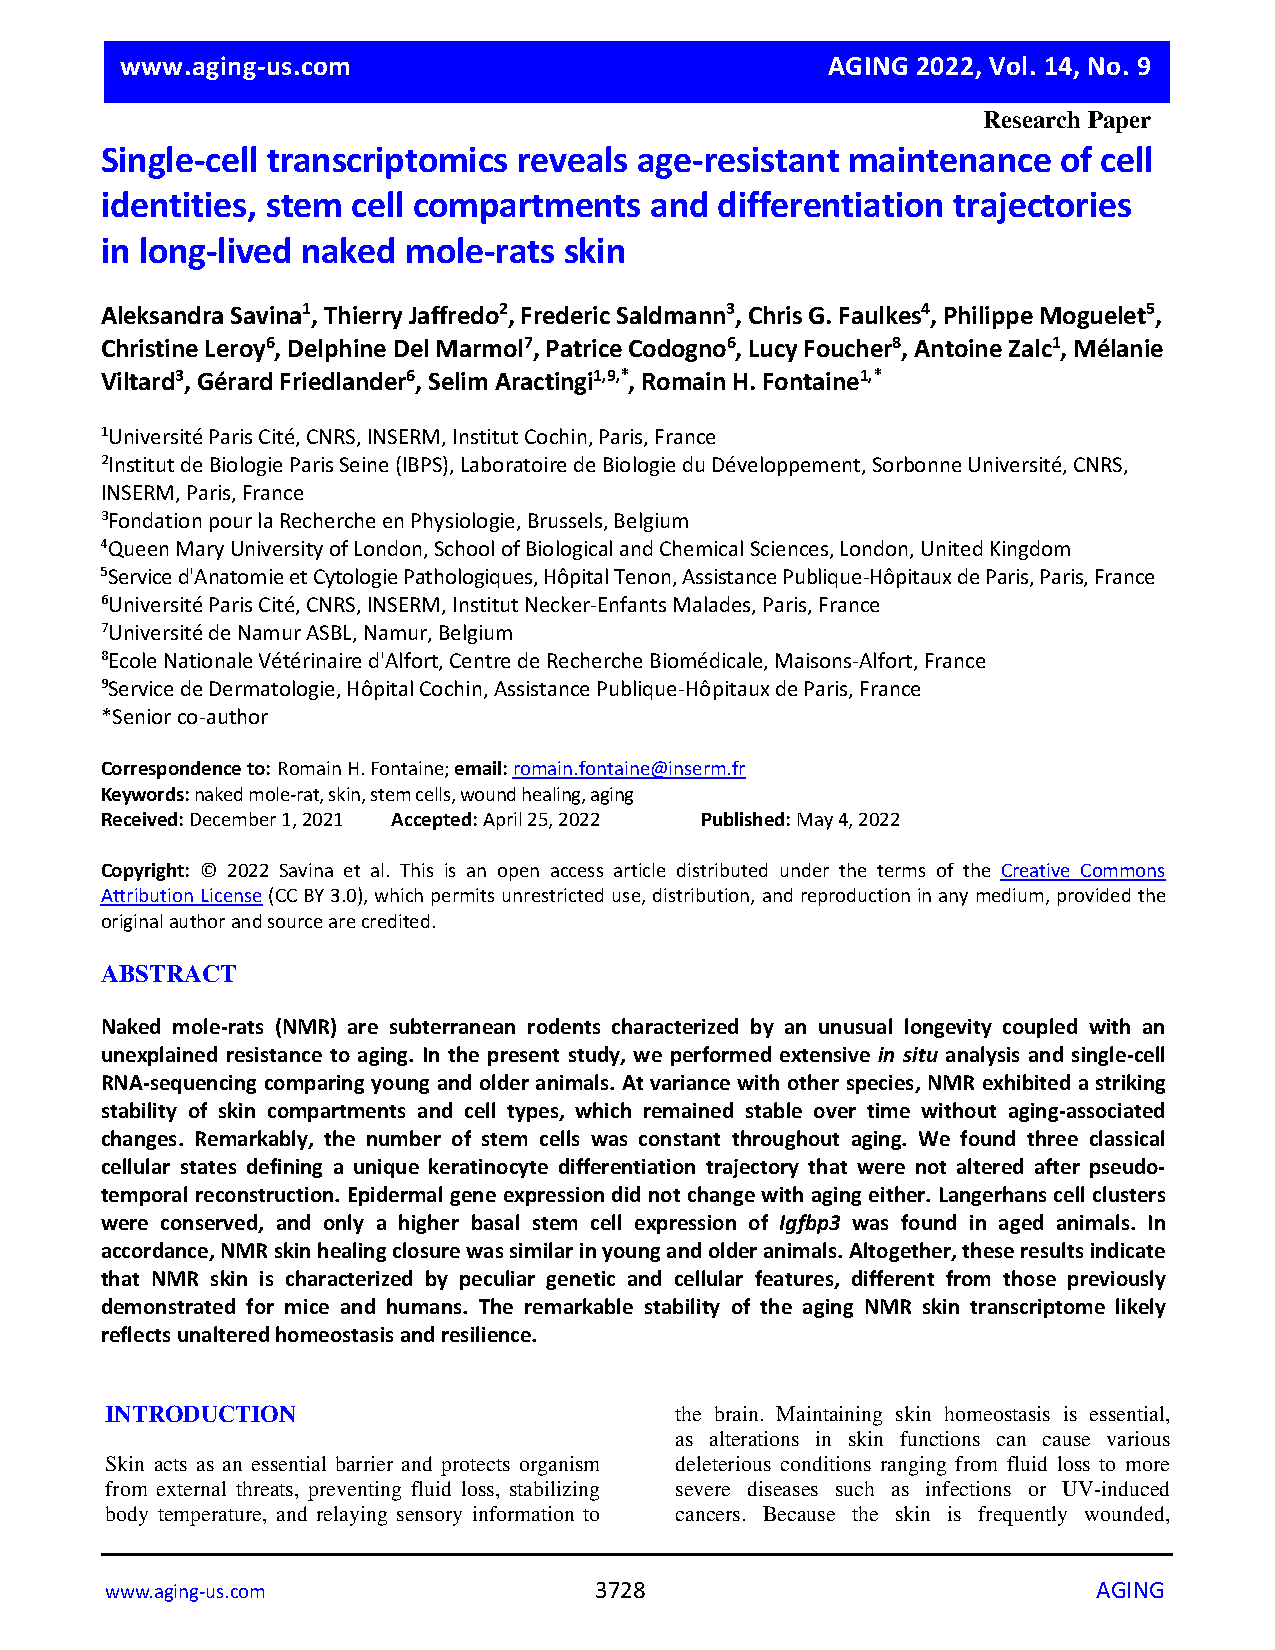
\includepdf[pages=-]{myfile.pdf}
%\chapter{Intitulé du chapitre}


\startcontents[chapters]

\textbf{Focus sur les articles dont vous êtes co-auteur et qui sont présentés dans votre thèse : vous devez les intégrer en texte intégral.
Introduisez chacun de vos articles par une page où vous indiquez le titre, les co-auteurs (sous la forme Prénom Nom), l’état (soumis, publié, etc.), ainsi que le nom de la revue et la date de publication s'il y a lieu.}


La différence majeure réside dans la présentation de la partie "contribution empirique" de la thèse sur articles qui est allégée par rapport à la thèse classique puisqu’il suffit de rédiger une ou deux pages d'introduction pour chacun des articles (minimum 3) directement insérés dans le texte. Cependant, la partie empirique de la thèse sur articles n'est pas une juxtaposition d'articles, elle doit constituer un ensemble cohérent et original qui permet d'apprécier la démarche de recherche de l'ensemble et la contribution du doctorant.


Les consignes sont les mêmes pour la thèse sur articles, à l'exception des articles qui seront insérés
dans le format et la langue dans lesquels ils ont été publiés ("pdf" des articles).

\section{section 1}

Un.e co-auteur.e du ou de l'un des articles présentés dans la thèse ne peut être rapporteur.e du travail de thèse.


\section{section 2}
\lipsum[2]

\subsection{subsection 1}
\lipsum[1]
\subsection{subsection 2}
\lipsum[1]

%\part*{Discussion et conclusion générale}
\fancyhead{} % clear all header fields
\fancyhead[OL]{\textsc{Discussion et perspectives}}
\chapter{Discussion et perspectives} % Main chapter title
%\addcontentsline{toc}{chapter}{Discussion et perspectives}  
%\pagestyle{plain} % remove headers/footers from the chapter page
%\startcontents[chapters]

%%%%%%%%%%%%%%--------------------%%%%%%%%%%%%%%%%%%%%%%%%%
%              ///  SECTION   \\\
%%%%%%%%%%%%%%--------------------%%%%%%%%%%%%%%%%%%%%%%%%%

%\section{Titre}


\newpage\thispagestyle{empty}

\fancyhead{} % clear all header fields
\fancyhead[OL]{\textsc{Conclusion}}
\chapter*{Conclusion générale} % Main chapter title
\markboth{Conclusion}{Conclusion}
\addcontentsline{toc}{chapter}{Conclusion générale}  
%\startcontents[chapters]
%\pagestyle{plain} % remove headers/footers from the chapt\markboth{Left}{Right}
 


%\pagestyle{fancy}
%\renewcommand{\chaptermark}[1]{\markboth{Chapter \thechapter. #1}{}}
%\renewcommand{\sectionmark}[1]{\markright{\thesection\ #1}}

\lipsum[40]

\lipsum[70]





\vspace{13pt}

Ainsi, l’ensemble des résultats présentés apportent des arguments en faveur de X.
\begin{itemize}[label=\textbullet]%[label=$\ast$]
        \item ta dignissim vestibulum, arcu diam lobortis velit, vel scelerisque risus augue sagittis risus. Maecenas eu justo. Pellentesque ha
        \item ta dignissim vestibulum, arcu diam lobortis velit, vel scelerisque risus augue sagittis risus. Maecenas eu justo. Pellentesque ha
        \item ta dignissim vestibulum, arcu diam lobortis velit, vel scelerisque risus augue sagittis risus. Maecenas eu justo. Pellentesque ha
\end{itemize}

\vspace{13pt}

Par conséquent, la poursuite de ces études devrait permettre de ta dignissim vestibulum, arcu diam lobortis velit, vel scelerisque risus augue sagittis risus. Maecenas eu justo.

\lipsum[70]

\lipsum[70]

\lipsum[70]

\lipsum[70]

\lipsum[70]

\lipsum[70]

\lipsum[70]

\lipsum[70]



%----------------------------------------------------------------------------------------
%	BIBLIOGRAPHY
%----------------------------------------------------------------------------------------
%\printbibliography %Prints bibliography
\fancyhead{} % clear all header fields
\fancyhead[OL]{\textsc{Bibliographie}}
\printbibliography[
heading=bibintoc,
title={Bibliographie "Adaptez le style bibliographique en fonction de votre discipline"}]

%----------------------------------------------------------------------------------------

%: ----------------------- glossary ------------------------
%\printindex
%\fancyhead{} % clear all header fields
%\fancyhead[OL]{\textsc{Glossaire}}
%\printglossary[title=Glossaire,toctitle=Glossaire]

%\input{auxilliaires/glossaire} 


\end{document}  
